\section{Discussion and conclusions}
\label{sec:results}

\subsection{Discussion of results}


As detailed above, this research aimed to establish a reliable model for classifying tissue section images. Initially, simple CNN models were implemented, but upon observing limited success, the study shifted towards image preprocessing and finally settled on transfer learning with the InceptionV3 model, which produced the best results.

It is worth noting that with the trial of different models, as the model parameters are adjusted or the model architecture becomes more complex (such as InceptionV3), the model's performance significantly improves, i.e., the accuracy of the validation set becomes higher and the loss becomes lower.

Furthermore, comparing model series 1 and 2, we found that using preprocessed images to assist the machine in extracting features is not very effective in the task of image classification. Image processing may lead to the loss of important details and information, thereby affecting the machine's feature extraction, and thus affecting the accuracy and performance of the model.

In Section 5, we tested the model in application. First, we selected an additional test set to test the model's accuracy and found that the model's accuracy on all test sets was greater than 85\%. Then we used the model to evaluate different cutting angles and found that if the cutting quality is to be guaranteed at 80\%, the cutting angle should be between 9 degrees and 10.5 degrees. Finally, we used another dataset of fish alveolar slice images for secondary verification and found that the model's prediction accuracy for the test set labels was all above 90\%, reflecting that the model can be well applied to other datasets.

The Final selected model configuration, illustrated below, highlights the structured approach taken to integrate the InceptionV3 architecture effectively within the training framework.

\begin{center}

    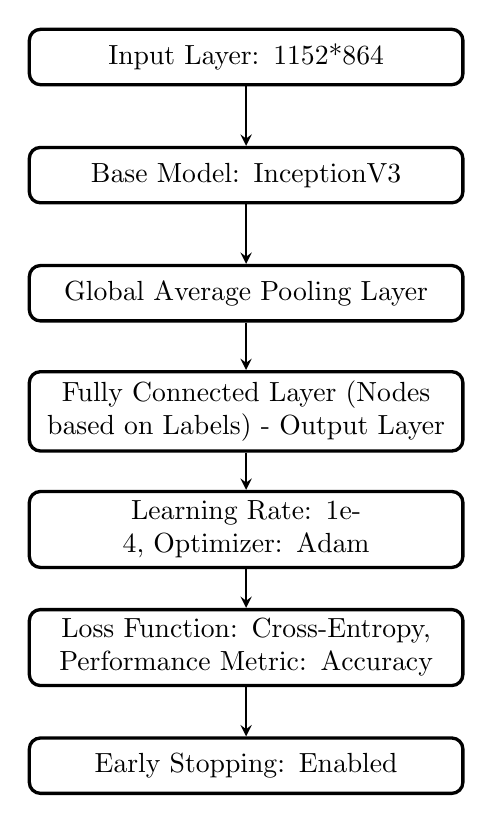
\begin{tikzpicture}[node distance=1.5cm,
        box/.style={
            rectangle,
            rounded corners,
            draw=black, very thick,
            text width=15em,
            minimum height=2em,
            text centered},
        arrow/.style={
            thick,
            ->,
            >=stealth}
        ]
    
        \node (collect) [box] {Input Layer: 1152*864};
        \node (mix) [box, below of=collect] {Base Model: InceptionV3};
        \node (train) [box, below of=mix] {Global Average Pooling Layer};
        \node (test) [box, below of=train] {Fully Connected Layer (Nodes based on Labels) - Output Layer};
        \node (evaluate) [box, below of=test] {Learning Rate: 1e-4, Optimizer: Adam};
        \node (rate) [box, below of=evaluate] {Loss Function: Cross-Entropy, Performance Metric: Accuracy};
        \node (improve) [box, below of=rate] {Early Stopping: Enabled};
        
        \draw [arrow] (collect) -- (mix);
        \draw [arrow] (mix) -- (train);
        \draw [arrow] (train) -- (test);
        \draw [arrow] (test) -- (evaluate);
        \draw [arrow] (evaluate) -- (rate);
        \draw [arrow] (rate) -- (improve);
        
        \end{tikzpicture}
\end{center}

\subsection{Future work}

\subsubsection{Enhancing Classification Methods}

\textbf{Broadening Classification Categories}

Current research shows promising outcomes using existing classification methods; however, these methods are confined to five categories. Expanding these categories could deepen insights into the correlation between cutting angles and sample quality, enhancing analytical precision. A broader classification spectrum could also improve predictions of optimal cutting angles for diverse tissue types and conditions.

\textbf{Transitioning to Linear Analytical Methods}

Introducing a more detailed classification could enable a shift from categorical to linear analytical methods. With sufficient categories acting as discrete points, linear relationships can be formed, allowing linear regression to accurately model the connection between cutting angles and sample quality.

Linear Discriminant Analysis (LDA) is valuable here, particularly for refining the determination of optimal cutting angles and correlating them with tissue quality. This approach simplifies predicting cutting parameters and enhances control over the tissue sectioning process.

\textbf{Challenges and Considerations}

Switching to a linear discriminant analysis framework poses significant challenges. Unlike binary classification models that provide probabilities, linear regression models explore direct relationships between variables, such as between cutting angles and tissue quality, which may not be straightforwardly linear.

Moreover, linear models require substantially more data, increasing both the duration and complexity of data collection and demanding greater computational resources. Current setups using TensorFlow and InceptionV3 models are already taxing GPU capacities, indicating a need for more advanced hardware and computational capabilities.

\textbf{Long-term Goals and Resource Needs}

These advancements are long-term objectives that require extensive resources and time. Research into linear discriminant analysis necessitates further theoretical study and practical experimentation. For instance, Jie Wen's "Robust Sparse Linear Discriminant Analysis" integrates sparsity into the LDA model, enhancing its robustness and suitability for complex applications.

% (如果可以增加相关论文证明观点:二分类和线性回归问题的对比和性能开销)


\subsubsection{Performance Enhancement and Optimization}

As this research progresses towards large-scale application, performance optimization emerges as a crucial challenge. This involves not only enhancing algorithm efficiency but also improving the scalability, stability, and deployment capabilities of the model framework, as well as optimizing the underlying programming languages and code.

To optimize the use of computational resources, adopting more efficient computing frameworks and parallel processing algorithms is essential. Utilizing distributed computing resources can significantly reduce model training times and enhance efficiency when processing large datasets. Moreover, considering constraints on energy consumption and computational costs, it's vital to optimize the model's computational architecture and parameter settings to maximize output within limited resources.

The article "Analysis of the Application Efficiency of TensorFlow and PyTorch in Convolutional Neural Network" highlights the differences between TensorFlow and PyTorch in processing convolutional neural networks\cite{6.2}. TensorFlow exhibits a lower error rate and smaller convergence steps, whereas PyTorch offers faster training speeds.

Pascal Fua's "Comparing Python, Go, and C++ on the N-Queens Problem" presents methods to optimize deep learning performance by comparing the efficiency of Python, Go, and C++ in solving the N-Queens problem.\cite{6.3} It was found that runtime languages have clear advantages in handling loops and data flows, suggesting that compiling tools like Numba, Cython, and Pybind11 can enhance performance in deep learning applications.




\subsubsection{Exploring the Impact of Additional Parameters on Cutting Quality}

In previous experiments, we established a model by setting the cutting angle as the independent variable and the cutting quality as the dependent variable. However, in reality, cutting quality may be influenced by other parameters such as cutting speed, feed rate (chip thickness), and tool wear.

In future work, if our focus is on the factors affecting cutting quality, research on these additional variables will be necessary. Indeed, the impact of these parameters on quality can be intuitively represented by a function:

\begin{equation}
Q = f(\theta, v, f, w)
\end{equation}

Here, $Q$ represents cutting quality, $\theta$ denotes the cutting angle, $v$ indicates the cutting speed, $f$ stands for the feed rate, and $w$ symbolizes tool wear. As for the specific form of this function, i.e., the weights of each parameter, it will require extensive experimental data for statistical analysis and fitting. This represents yet another challenge.

\subsubsection{Optimization of the Sectioning Process}

Our research also uncovered that real-time assessment of section quality during the cutting process, followed by adjustments based on those assessments, could significantly improve the quality of tissue sections.

The proposed feedback adjustment process involves installing a camera above the microtome to capture data from the samples being cut. This data is then analyzed in real-time by a pre-trained model, which assesses the quality of the sections. Based on this assessment, the cutting speed and angle parameters of the microtome can be adjusted to improve the quality of subsequent sections, thus ensuring controllable and consistent sample quality.

Implementing this system presents several challenges:

\begin{itemize}
    \item \textbf{Real-Time Image Processing:} A clear camera and an efficient real-time image processing system are needed to capture and process image data swiftly.
    \item \textbf{Powerful Computing Resources:} A pre-trained model and a powerful computer are required to quickly assess images and adjust the microtome's parameters based on the assessment.
    \item \textbf{Effective Control Interface:} An efficient control interface is necessary to ensure that the adjusted parameters are promptly communicated to the microtome.
    \item \textbf{Time Efficiency:} The entire system must operate within the brief intervals between cuts.
\end{itemize}

A pertinent example can be found in the study "Convolutional neural networks applied to microtomy: Identifying the trimming-end cutting routine on paraffin-embedded tissue blocks"\cite{6.4}. This research automated the sectioning process by monitoring it with a camera, analyzing the images with a CNN, and adjusting the microtome parameters based on the analysis. This integration of the microtome, camera, and deep learning model provides a feasible solution for real-time assessment and adjustment of cutting parameters during the sectioning process.


\subsection{Conclusions}

This research has significantly advanced our understanding of optimizing biopsy parameters through the application of deep learning techniques to biomedical tissue sectioning devices. By employing sophisticated convolutional neural networks, particularly through the adaptation of the InceptionV3 model via transfer learning, the study has demonstrated a robust framework capable of assessing the quality of tissue sections with high precision. This approach not only improves the accuracy of tissue sample analysis but also introduces a paradigm shift in the operational methodology of tissue sectioning.

By evaluating the quality of sections at different angles, we have discovered the relationship between the cutting angle and the quality of the sections. This provides us with a feasible method to improve the quality of sections in the future. In addition, the application of this model in different types of tissues (including fish ovaries and lung tissues) has confirmed its wide adaptability and potential for promotion, indicating that it is suitable for various tissue sections and research tasks.

However, the study also highlighted the limitations of traditional image preprocessing techniques. Initial attempts to enhance model performance through image preprocessing did not yield significant improvements and, in some cases, potentially obscured critical details necessary for accurate classification. This finding suggests that maintaining the integrity of original image data might be more beneficial than applying aggressive preprocessing techniques.

The research further explores enhancing the tissue slicing process through the expansion of classification methods and performance optimization. This includes integrating a greater number of classification categories and linear analysis methods such as Linear Discriminant Analysis (LDA), to more precisely understand the relationship between cutting parameters and sample quality. Concurrently, adopting more efficient computational frameworks and parallel processing techniques to optimize performance, as well as exploring additional parameters such as cutting speed and feed rate, will enhance the predictive capability of the model and the quality of tissue slices. Moreover, the implementation of a real-time feedback system, utilizing machine learning to dynamically adjust cutting parameters, will propel histological preparation towards automation, ensuring more consistent and high-quality tissue slices.

In conclusion, this project not only demonstrates the important role of deep learning in biomedical research and applications, but also provides feasibility for the further improvement of tissue sectioning technology. The combination of these technologies can bring improvements to biological sectioning equipment, provide a possible solution to improve the yield rate of tissue samples and the efficiency of sectioning. This research provides new ideas and methods for future tissue sectioning technology, and is expected to have a profound impact in the field of biomedicine.

% 总之,该项目不仅体现了深度学习在生物医学研究和应用中的重要作用,而且为组织切片技术的进一步提高提供了可行性。将这些技术的有机结合能够为生物切片设备带来改进,提高组织样本的良品率及提高切片效率提供了一个可能的解决方案。这一研究为未来的组织切片技术提供了新的思路和方法,有望在生物医学领域产生深远的影响。

\FloatBarrier % Now the table doesn't flow over to any other sections